\clearpage
\item \points{40} {\bf Linear Classifiers (logistic regression and GDA)}

In this problem, we cover two probabilistic linear classifiers we have
covered in class so far. First, a discriminative linear classifier: logistic
regression. Second, a generative linear classifier: Gaussian discriminant
analysis (GDA). Both the algorithms find a linear decision boundary that
separates the data into two classes, but make different assumptions. Our goal
in this problem is to get a deeper understanding of the similarities and
differences (and, strengths and weaknesses) of these two algorithms.

For this problem, we will consider two datasets, provided in the following
files:
\begin{enumerate}[label=\roman*.]
	\item \url{data/ds1_{train,valid}.csv}
	\item \url{data/ds2_{train,valid}.csv}
\end{enumerate}
Each file contains $m$ examples, one example $(x^{(i)}, y^{(i)})$ per row.
In particular, the $i$-th row contains columns $x^{(i)}_0\in\Re$,
$x^{(i)}_1\in\Re$, and $y^{(i)}\in\{0, 1\}$. In the subproblems that follow, we
will investigate using logistic regression and Gaussian discriminant analysis
(GDA) to perform binary classification on these two datasets.

\begin{enumerate}
	\item \subquestionpoints{5}
Show that the above property holds true for the described logistic regression
model over the range $(a,b) = (0,1)$.

\textit{Hint}: Use the fact that we include a bias term.

\ifnum\solutions=1 {
  \begin{answer}

The gradient of the log likelihood is given by:

$$
    l(\theta) = X^T(\vec{y} - g(X\theta))
$$

    For the best $\theta$, we will have $X^T\vec{y} = X^Th_\theta(X)$. If we only consider the first row of $X^T$, we will find

    $$
    \sum_{i=1}^my^{(i)} = \sum_{i=1}^m h_\theta(x^{(i)})
    $$
which directly shows the result we want to prove.
\end{answer}

} \fi

	\clearpage
\item \subquestionpoints{5} \textbf{Coding problem.}
Follow the instructions in \texttt{src/p01b\_logreg.py} to train a
logistic regression classifier using Newton's Method.
Starting with $\theta = \vec{0}$, run Newton's Method until the updates to
$\theta$ are small: Specifically,  train until the first iteration $k$ such
that $\|\theta_{k} - \theta_{k-1}\|_1 < \epsilon$, where
$\epsilon = 1\times 10^{-5}$. Make sure to write your model's predictions to
the file specified in the code.

\ifnum\solutions=1 {
  \begin{answer}
\end{answer}

} \fi

	\clearpage
\item \subquestionpoints{5}
Recall that in GDA we model the joint distribution of $(x, y)$ by the following
equations:
%
\begin{eqnarray*}
	p(y) &=& \begin{cases}
	\phi & \mbox{if~} y = 1 \\
	1 - \phi & \mbox{if~} y = 0 \end{cases} \\
	p(x | y=0) &=& \frac{1}{(2\pi)^{n/2} |\Sigma|^{1/2}}
		\exp\left(-\frac{1}{2}(x-\mu_{0})^T \Sigma^{-1} (x-\mu_{0})\right) \\
	p(x | y=1) &=& \frac{1}{(2\pi)^{n/2} |\Sigma|^{1/2}}
		\exp\left(-\frac{1}{2}(x-\mu_1)^T \Sigma^{-1} (x-\mu_1) \right),
\end{eqnarray*}
%
where $\phi$, $\mu_0$, $\mu_1$, and $\Sigma$ are the parameters of our model.

Suppose we have already fit $\phi$, $\mu_0$, $\mu_1$, and $\Sigma$, and now
want to predict $y$ given a new point $x$. To show that GDA results in a
classifier that has a linear decision boundary, show the posterior distribution
can be written as
%
\begin{equation*}
	p(y = 1\mid x; \phi, \mu_0, \mu_1, \Sigma)
	= \frac{1}{1 + \exp(-(\theta^T x + \theta_0))},
\end{equation*}
%
where $\theta\in\Re^n$ and $\theta_{0}\in\Re$ are appropriate functions of
$\phi$, $\Sigma$, $\mu_0$, and $\mu_1$.

\ifnum\solutions=1{
  \begin{answer}
We have
$$
\begin{aligned}
p(y=1|x, \phi, \mu_0, \mu_1, \Sigma) &= \frac{p(x|y=1)p(y=1)}{p(x|y=1)p(y=1) + p(x|y=0)p(y=0)}\\
&= \frac{1}{1 + \frac{p(x|y=0)p(y=0)}{p(x|y=1)p(y=1)}}\\
&= \frac{1}{1 + \exp(-\frac{1}{2}[(x - \mu_0)^T\Sigma^{-1}(x - \mu_0) -(x - \mu_0)^T\Sigma^{-1}(x - \mu_0)])}\frac{1 - \phi}{\phi}\\
&= \frac{1}{1 + \exp(-[(\mu_1 - \mu_0)^T\Sigma^{-1}x  ) + \frac{1}{2}(\mu_0^T\Sigma^{-1}\mu_0 - \mu_1^T\Sigma^{-1}\mu_1) - \log\frac{1-\phi}{\phi}]}
\end{aligned}
$$

So we can take 

$$
\theta = (\mu_1 - \mu_0)^T\Sigma^{-1},\\ 
\theta_0 = \frac{1}{2}(\mu_0^T\Sigma^{-1}\mu_0 - \mu_1^T\Sigma^{-1}\mu_1) - \log\frac{1-\phi}{\phi}
$$

\end{answer}

}\fi

	\clearpage
\item \subquestionpoints{7} For this part of the problem only, you may
  assume $n$ (the dimension of $x$) is 1, so that $\Sigma = [\sigma^2]$ is
  just a real number, and likewise the determinant of $\Sigma$ is given by
  $|\Sigma| = \sigma^2$.  Given the dataset, we claim that the maximum
  likelihood estimates of the parameters are given by
  \begin{eqnarray*}
    \phi &=& \frac{1}{m} \sum_{i=1}^m 1\{y^{(i)} = 1\} \\
\mu_{0} &=& \frac{\sum_{i=1}^m 1\{y^{(i)} = {0}\} x^{(i)}}{\sum_{i=1}^m
1\{y^{(i)} = {0}\}} \\
\mu_1 &=& \frac{\sum_{i=1}^m 1\{y^{(i)} = 1\} x^{(i)}}{\sum_{i=1}^m 1\{y^{(i)}
= 1\}} \\
\Sigma &=& \frac{1}{m} \sum_{i=1}^m (x^{(i)} - \mu_{y^{(i)}}) (x^{(i)} -
\mu_{y^{(i)}})^T
  \end{eqnarray*}
  The log-likelihood of the data is
  \begin{eqnarray*}
\ell(\phi, \mu_{0}, \mu_1, \Sigma) &=& \log \prod_{i=1}^m p(x^{(i)} , y^{(i)};
\phi, \mu_{0}, \mu_1, \Sigma) \\
&=& \log \prod_{i=1}^m p(x^{(i)} | y^{(i)}; \mu_{0}, \mu_1, \Sigma) p(y^{(i)};
\phi).
  \end{eqnarray*}
By maximizing $\ell$ with respect to the four parameters,
prove that the maximum likelihood estimates of $\phi$, $\mu_{0}, \mu_1$, and
$\Sigma$ are indeed as given in the formulas above.  (You may assume that there
is at least one positive and one negative example, so that the denominators in
the definitions of $\mu_{0}$ and $\mu_1$ above are non-zero.)

\ifnum\solutions=1 {
  \begin{answer}
We have
    $$
    \begin{aligned}
l(\phi, \mu_0, \mu_1, \Sigma) &= \sum_{i=1}^m(\log p(x^{(i)}|y^{(i)}; \mu_0, \mu_1, \Sigma) + \log p(y^{(i)};\phi))\\
&= \sum_{i=1}^m [1\{y^{(i)} = 0\} \log \frac{1}{\sqrt{2\pi}\sigma}\exp(-\frac{(x^{(i)} - \mu_0)^2}{2\sigma^2}) + 1\{y^{(i)} = 1\} \log \frac{1}{\sqrt{2\pi}\sigma}\exp(-\frac{(x^{(i)} - \mu_1)^2}{2\sigma^2}) + y^{(i)} \log \phi + (1 - y^{(i)}\log (1- \phi))]
\end{aligned}
$$
And we set derivatives to zero:

    \[
\begin{aligned}
\frac{\partial l}{\partial \phi} = y^{(i)}\frac{1}{\phi} + (1 - y^{(i)})\frac{1}{1- \phi} = 0\\
\frac{\partial l}{\partial \mu_0} = - \sum_{i=1}^m1\{y^{(i)} = 0\} \frac{x^{(i)} - \mu_0}{\sigma^2} = 0\\
\frac{\partial l}{\partial \mu_1} = - \sum_{i=1}^m1\{y^{(i)} = 1\} \frac{x^{(i)} - \mu_1}{\sigma^2} = 0\\
\frac{\partial l}{\partial \sigma^2 } = \sum_{i=1}^m -\frac{1}{2\sigma^2} + \frac{(x^{(i)} - \mu_{y^{(i)}})^2}{2\sigma^4} = 0
\end{aligned}
\]
And from these we get the estimations.
\end{answer}


} \fi

	\clearpage
\item \subquestionpoints{3} \textbf{Coding problem.}
In \texttt{src/p01e\_gda.py}, fill in the code to
calculate $\phi$, $\mu_{0}$, $\mu_{1}$, and $\Sigma$, use these parameters
to derive $\theta$, and use the resulting GDA model to make predictions on the
validation set.

\ifnum\solutions=1 {
  \begin{answer}
\end{answer}

} \fi

	\clearpage
\item \subquestionpoints{5}
For Dataset 1, create a plot of the training data with $x_1$ on the horizontal
axis, and $x_2$ on the vertical axis. To visualize the two classes, use a
different symbol for examples $x^{(i)}$ with $y^{(i)} = 0$ than for those with
$y^{(i)} = 1$. On the same figure, plot the decision boundary found by logistic
regression in part (b). Make an identical plot with the decision boundary found
by GDA in part (e).

\ifnum\solutions=1 {
\begin{answer}
\begin{figure}[htbp]
    \begin{subfigure}[b]{0.5\linewidth}
        \centering
        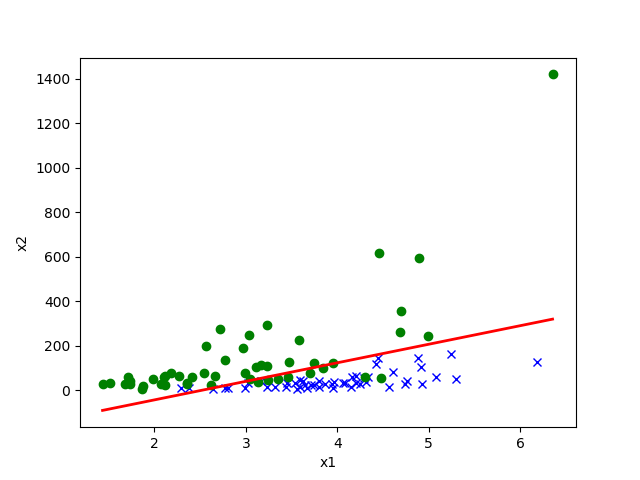
\includegraphics[width=\linewidth]{pics/p01b_1.png}
        \subcaption{Logistic Regression on Dataset 1}
    \end{subfigure}
    \begin{subfigure}[b]{0.5\linewidth}
        \centering
        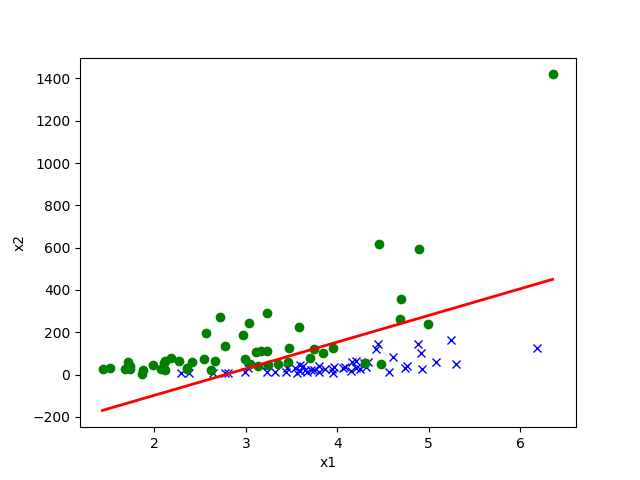
\includegraphics[width=\linewidth]{pics/p01e_1.png}
        \subcaption{GDA on Dataset 1}
    \end{subfigure}

\end{figure}

\end{answer}

} \fi

	\clearpage
\item \subquestionpoints{5}
Repeat the steps in part (f) for Dataset 2. On which dataset does GDA seem to
perform worse than logistic regression? Why might this be the case?

\ifnum\solutions=1{
  \begin{answer}
\begin{figure}[htbp]
    \begin{subfigure}[b]{0.5\linewidth}
        \centering
        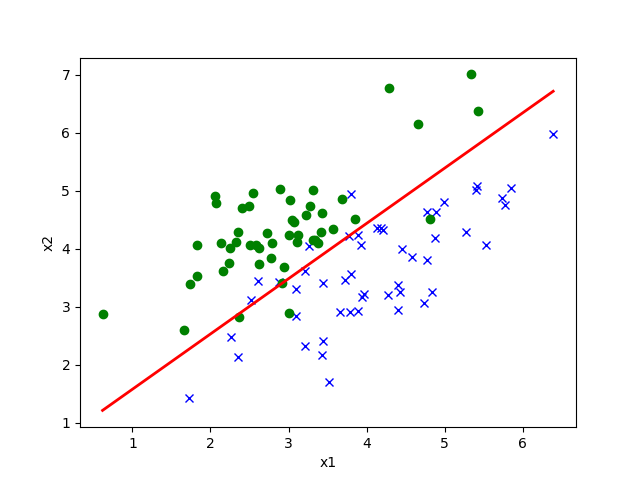
\includegraphics[width=\linewidth]{pics/p01b_2.png}
        \subcaption{Logistic Regression on Dataset 2}
    \end{subfigure}
    \begin{subfigure}[b]{0.5\linewidth}
        \centering
        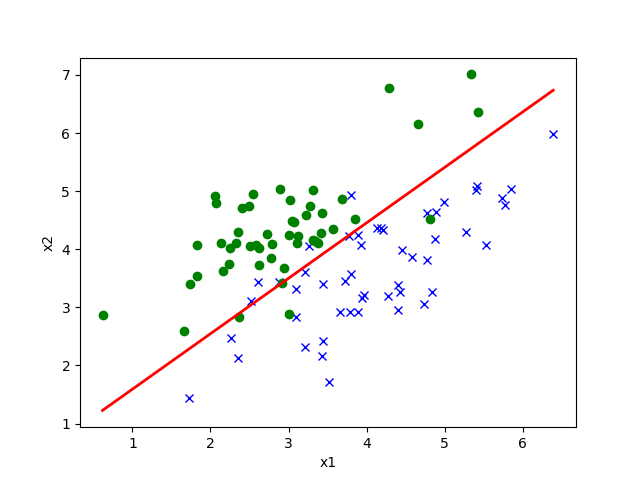
\includegraphics[width=\linewidth]{pics/p01e_2.png}
        \subcaption{GDA on Dataset 2}
    \end{subfigure}

\end{figure}

On dataset1. This is because the distribution of data given label is not gaussian.

\end{answer}

}\fi

	\clearpage
\item \points{3 extra credit} For the dataset where GDA performed worse in
parts (f) and (g), can you find a transformation of the $x^{(i)}$'s such
that GDA performs significantly better? What is this transformation?

\ifnum\solutions=1{
  \begin{answer}
Maybe using a log transformation.
\end{answer}

}\fi

\end{enumerate}
